\documentclass{article}
\usepackage[utf8]{inputenc}
\usepackage{graphicx,wrapfig,lipsum}

\usepackage{amssymb}
\usepackage{amsmath}
\usepackage{subfigure}
\usepackage{geometry}
\newcommand{\euler}{e}
\newcommand{\ramuno}{i}
\def\MA#1{{\color{blue}#1}}
\def\bs#1{\boldsymbol{#1}}
% proportions du docc
 \geometry{
 a4paper,
 total={170mm,257mm},
 left=20mm,
 top=20mm,
 }
 
 
\title{Projet : modélisation de pics de production de ressources }
\author{Yoan Thomas\and  Aya Ismahene Kroussa\and Melvin Cerba}

\begin{document}
% Page de garde
\begin{figure}
        \center
        
\includegraphics[scale = 0.4]{graphes/fig1.png}
\end{figure}
\maketitle
\begin{figure}[h]
        \center
        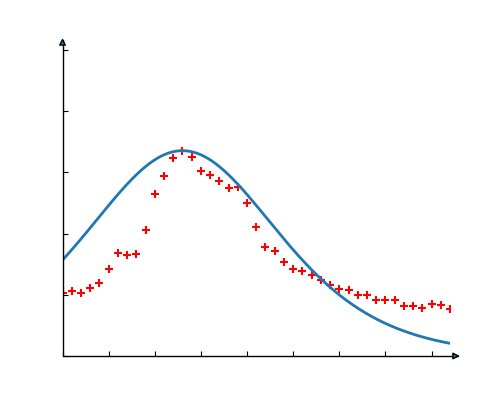
\includegraphics[scale = 1]{graphes/Courbe_de_Hubbert_Data.png}
\end{figure}


% Sommaire
\newpage
\vspace*{\fill}
\tableofcontents
\vspace*{\fill}


%
\newpage

\section{Élément historique}
% Explication des motivations du rapport %
$\indent$ Peut-on prédire l'évolution de la production des ressources non renouvelables ? Pour tenter de répondre à cette question, nous proposons d'étudier à travers ce projet certains outils mathématiques qui permettent de modéliser la production des ressources non renouvelables. Plus spécifiquement, nous nous intéresserons à la production de pétrole.



\subsection{Modélisation des pics de productions}
% Contexte historique et pratique %
\begin{wrapfigure}{r}{5.5cm}
	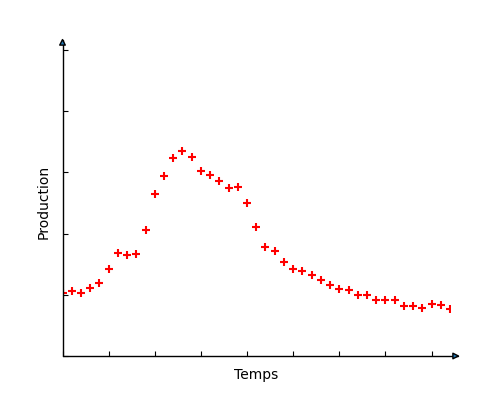
\includegraphics[width=5.5cm]{graphes/Production.png}
	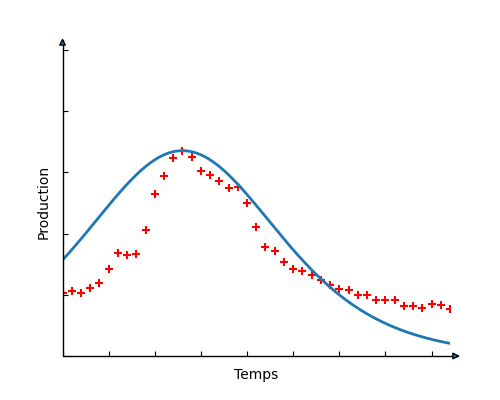
\includegraphics[width=5.5cm]{graphes/DataEtHubbert.png}
\end{wrapfigure} 
$\indent$ Être capable de prédire l'évolution de la production de diverses ressources a toujours été un enjeu majeur, notamment en économie. Il est donc naturel que de nombreux modèles mathématiques promettant de modéliser cette évolution soient apparus. A travers ce projet, nous vous proposons d'étudier en détail l'un d'eux : la courbe de Hubbert. \\
$\indent$ En 1956, Marion King Hubbert présentait sa "courbe de Hubbert" à l'American Petroleum Institute. Son modèle, qui postule que la production  croit, atteint un unique pic, puis décroit au même rythme qu'elle a augmenté en premier lieu, ne fit pas beaucoup parler de lui à l'époque. Mais lorsqu'en 1971, conformément à ses prédictions, la production pétrolière américaine atteignit son maximum et commença à décliner, ses travaux furent réexaminés avec beaucoup plus d'intérêt. Les chocs pétroliers de 1973 et 1979 semblèrent cependant définitivement invalider son modèle, qui perdit rapidement l'attention de l'industrie pétrolière.  \\
$\indent$ Malgré tout, l'avènement du calcul informatique et la grande disponibilité de données poussèrent des auteurs modernes à exhumer le modèle de Hubbert et à l'étendre, notamment en donnant une formule mathématique à sa courbe, permettant ainsi de calculer son intégrale. C'est sur la base de ces nouveaux travaux que nous avons construit notre projet.\\ \\



\subsection{Courbe de Hubbert et sigmoïde}
% Introduction du modèle mathématique et explication des paramètres %
$\indent$ Les auteurs qui se sont rapproprié la courbe de Hubbert ont notamment travaillé à lui donner une expression mathématique. Ceci leur a permis de définir son intégrale, que nous appellerons "fonction sigmoïde" tout au long de ce rapport. Pour des raisons que nous expliciterons plus bas, cette dernière s'avère plus facile à manier que la courbe de Hubbert.\\


\begin{figure}[h]
	\centering
    \subfigure{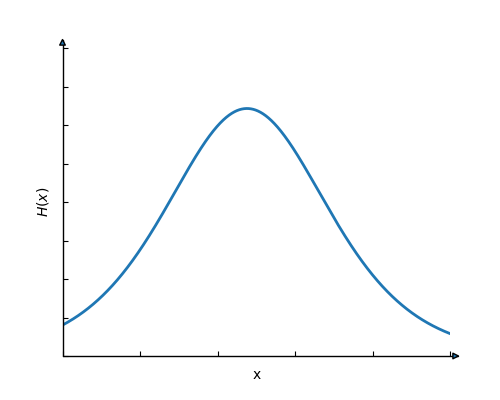
\includegraphics[width=0.40\textwidth]{graphes/CourbeHubbert.png}}
    \subfigure{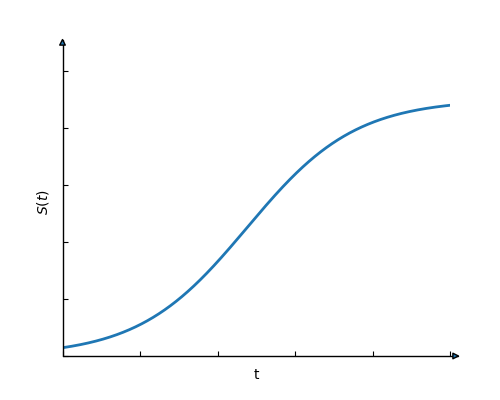
\includegraphics[width=0.40\textwidth]{graphes/Sigmoide.png}}
    \caption{Une courbe de Hubbert et sa sigmoïde (son intégrale)}
    %\label{fig:foobar}
\end{figure}:\\


%$\indent$
Une \textit{courbe de Hubbert}\footnote{
Page wikippédia $\bullet$ Nuclear energy and the fossil fuels [archive] M. King Hubbert, $1956$\\
$~~~~~~~$ $\bullet$The Hubbert parabola [archive], Roberto Canogar
}
est une courbe qui décrit de manière explicite l'évolution au cours du temps de la production d'une ressource donnée (par exemple, du pétrole). Cette fonction s'écrit
  %
  \begin{equation}\label{linspring_1}
    H(t;  \boldsymbol{\theta}) =  \frac{S_{\max}}{\tau}\frac{ e^{-\frac{t-t_\star}{\tau}}}{\left(1+ e^{-\frac{t-t_\star}{\tau}}\right)^2}
    \qquad
    \begin{gathered}
      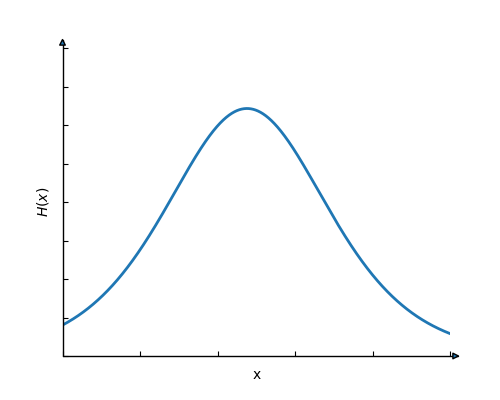
\includegraphics[width=0.40\textwidth]{graphes/CourbeHubbert.png}
    \end{gathered}
\end{equation}
%
Dans l'expression ci-dessus, $t$ représente la variable de temps et le
triplet de paramètre paramètres $\boldsymbol{\theta} := (S_{\text{max}}, t_\star,\tau)$
permet de  définir sans ambigüité la courbe dans la famille paramétrée.
%
Comme le montre l'illustration ci-dessus, cette courbe à la forme
d'une ``cloche'' et les trois paramètres définissent son allure
générale. Plus spécifiquement, on a
%
\begin{itemize}
\item $S_{\text{max}}$ contrôle l'amplitude maximale de la courbe ;
\item $t_\star$ repère la position de ce maximum sur l'axe des temps  ;
  \item $\tau$ contrôle le caractère plus ou moins ``piqué'' de la cloche.
\end{itemize}
%
L'intégrale de cette fonction de Hubbert possède la forme explicite
suivante :
%
\begin{equation}\label{linspring_2}
  S(t; \boldsymbol{\theta}) =\frac{S_{\text{max}}}{1+  e^{\frac{-(t-t_\star)}{\tau}}}
  \qquad
  \begin{gathered}
    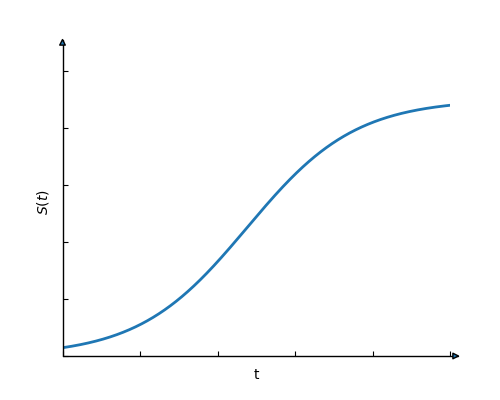
\includegraphics[width=0.40\textwidth]{graphes/Sigmoide.png}
  \end{gathered}
\end{equation}
%
Cette fonction est largement connue sous le nom de \textit{fonction
  sigmoïde}. Dans le cadre d'une interprétation de la consommation
de ressources naturelles, la sigmoïde modélise l'évolution temporelle
\textit{cumulée} de ressource extrait du sol.

$\indent$ Rappelons notre objectif et nos hypothèses : nous voulons modéliser la production de pétrole au cours du temps, et nous supposons que celle-ci atteint un unique pic. Il nous faudra donc déterminer le $t$ pour lequel ce pic est atteint ainsi que la hauteur de ce pic (quantité de pétrole produit à l'instant $t$).

\begin{figure}[h]
	\centering
    \subfigure{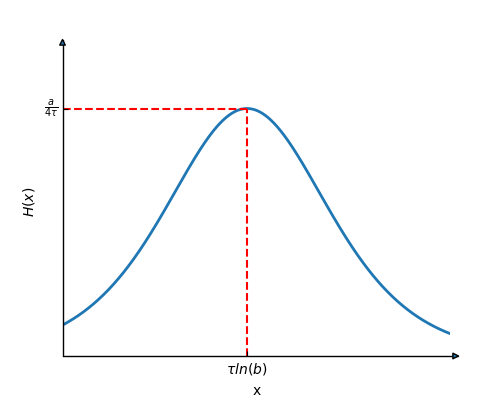
\includegraphics[width=0.45\textwidth]{graphes/Courbe_de_Hubbert_annotée.png}} 
    \subfigure{\includegraphics[width=0.45\textwidth]{graphes/SigmoideAnnotée.png}} 
    \caption{Une courbe de Hubbert et sa sigmoïde ($\Delta$ : pente de la sigmoïde au point d'inflexion $t_*$) }
    %\label{fig:foobar}
\end{figure}


\newpage






\section{Algorithme d'approximation}
% Explication de l'algorithme et des mathématiques sous jacentes %
$\indent$ Afin d'approximer les paramètres de la sigmoide la plus en adéquation avec nos données, nous allons utiliser une méthode de minimisation de fonction réputée : la \textit{descente de gradient}.\\
\\

$\indent$ \textbf{Conditions à vérifier}
\begin{itemize}
\item \textit{Initialisation :} pour que l'algorithme "descende" vers le minimum absolu de la fonction, il faut l'initialiser dans un "creux" qui le contienne, c'est à dire un intervalle sur lequel la fonction est convexe et dont l'image contient le minimum absolu de la fonction.
\item \textit{Direction de descente :} par ailleurs, il faut être certain que l'algorithme sache en tout instant dans quelle direction aller (ie. quelles modifications apporter aux paramètres) pour "descendre" vers le minimum. Pour cela, nous utiliserons le gradient. 
\end{itemize}

$\indent$\textbf{Algorithme}\\
$\indent$ L'algorithme fonctionne de la manière suivante : 
\begin{enumerate}
\item Il calcule $\bs{\nabla}\text{Crit}_{\text{D}}(S(t; \boldsymbol{\theta}))$ le gradient de la fonction critère.
\item Il définit une direction de descente $d$ à partir de $\bs{\nabla}C$.
\item Il modifie les paramètres initiaux selon $d$ et un pas $\delta t$.
\item Puis il recommence, jusqu'à satisfaire des conditions prédéfinies qui assure une certaine proximité au minimum de la fonction.
\end{enumerate}


\subsection{Caractérisation}
% Explication détaillées de chaque parties de l'algorithme %
$\indent$ Dans cette partie, nous 



\subsubsection{Critère}
% Explication du critère à optimiser %
$\indent$ Avant toute chose, il nous faut une fonction à minimiser. Nous allons donc définir un \textit{critère} qui évalue la distance qui sépare les données de la courbe du modèle. Plus précisément, nous additionnerons pour chaque année le carré de la différence entre l'estimation du modèle et les données réelles.
\begin{equation}\label{eqn:eqCrit}
	Criterion_{Data}(Sig(t;\Theta )) = \sum_{k=1}^{N} \delta t | Data(t_k) - Sig(t_k;\Theta ) |^2
\end{equation}
$\indent$ avec :
\begin{center}
	$Data(t_k)$ la somme des données de production de l'instant $t_1$ à l'instant $t_k$\\
 	$\delta t$ 
\end{center}
\textit{ Par la suite, on notera indifféremment $Criterion_{Data}(Sig(t;\Theta ))$, $Crit_D(Sig(t;\Theta ))$ ou $Crit(Sig(t;\Theta ))$.}


\subsubsection{Gradient}
% Calcule du gradient et de la jacobienne %
$\indent$ Afin de converger vers les paramètres optimaux, l'algorithme de la descente de gradient a besoin d'une direction de descente. Cela passe avant tout par le calcul du gradient de la fonction à minimiser, afin d'avoir une idée précise de l'évolution de cette dernière en fonction de chaque paramètre.\\
$\indent$ A partir de (\ref{eqn:eqCrit}), on obtient :

\begin{equation}\label{linspring}
	\nabla \text{Crit}(\text{S}(t;\boldsymbol{\theta } )) = \sum_{k=1}^{N} 2 *\nabla\text{ S}(t_k ;\boldsymbol{\theta }) * (\text{S}(t_k ;\boldsymbol{\theta } )- \text{D}(t_k))
\end{equation}

$\indent$ Il nous faut donc définir $\vec{\nabla} Sig(\Theta)$ :

$$
\vec{\nabla} Sig(t;\Theta)= \dfrac{\partial ^2 Sig}{\partial t \partial \Theta}(t,\Theta ) 
= \left[\begin{array}{c}
\dfrac{\partial Sig}{\partial t \partial S_{max}}(t,\Theta )\\
\\
\dfrac{\partial Sig}{\partial t \partial t_*}(t,\Theta ) \\
\\
\dfrac{\partial Sig}{\partial t \partial \tau}(t,\Theta ) 
\end{array}\right] 
$$

$\indent$ Par le calcul, on obtient :

\begin{equation}\label{linspring}
\large \vec{\nabla} Sig(t;\Theta) = \left[\begin{array}{c}
\frac{1}{1 + e^{-\frac{(t-t_*)}{\tau}}}\\
\\
\frac{- S_{max}}{\tau}*\frac{e^{-\frac{(t-t_*)}{\tau}}}{(1+e^{-\frac{(t-t_*)}{\tau}})^2} \\
\\
\frac{- S_{max}}{\tau ^2}*\frac{e^{-\frac{(t-t_*) * (t-t_*)}{\tau}}}{(1+e^{-\frac{(t-t_*)}{\tau}})^2}
\end{array}\right]
\end{equation}
\\
$\indent$ Nous sommes donc capables de calculer le gradient de la sigmoïde pour des paramètres $S_{max}$ , $t_*$ et $\tau$ donnés. Mais comment en tirer une direction de descente ? 


\subsubsection{Direction de descente}
% Définition de la direction de descente %
Le gradient nous d



\subsubsection{Figure des isocourbes avec les direction de descentes}
% Affichage de figure, et justification de la nécessité de l'utilisation d'une matrice de mise à l'échelle %
\textit{Affichage de figure, et justification de la nécessité de l'utilisation d'une matrice de mise à l'échelle}

\begin{figure}[h]
	\centering
    \subfigure{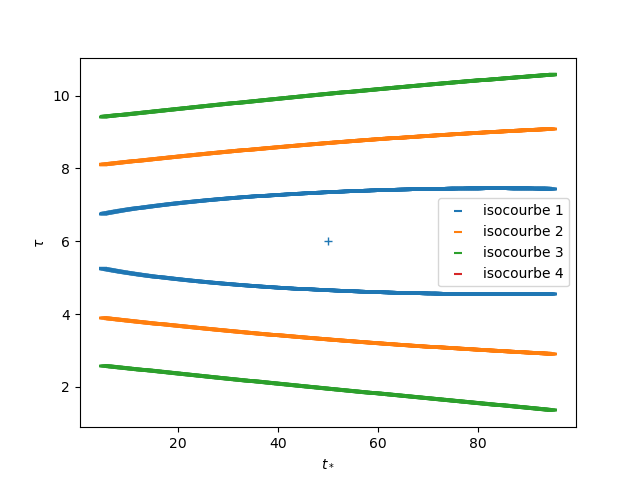
\includegraphics[width=0.33\textwidth]{graphes/isocurves_Smax.png}} 
    \subfigure{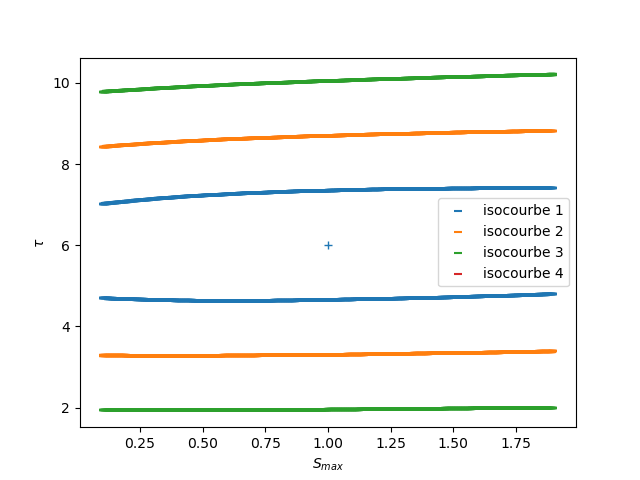
\includegraphics[width=0.33\textwidth]{graphes/isocurves_ts.png}} 
    \subfigure{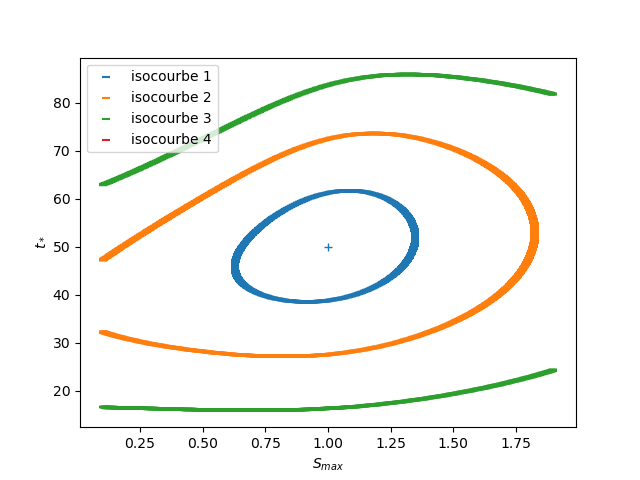
\includegraphics[width=0.33\textwidth]{graphes/isocurves_tau.png}} 
    \caption{Une courbe de Hubbert et sa sigmoïde ($\Delta$ : pente de la sigmoïde au point d'inflexion $t_*$) }
    %\label{fig:foobar}
\end{figure}



\subsubsection{Matrice de mise à l'échelle}
% Définition de la matrice de mise à l'échelle %
\textit{Définition de la matrice de mise à l'échelle}



\subsubsection{Pseudo code}
% Pseudo Code %
\textit{Pseudo code}



\subsection{Test de contrôle de l'algorithme et des fonctions associées}
% Avant de lancer la l'algorithme sur des données réelles on vérifie que nos fonctions soient justes et que l'algorithme converge pour des données simulées %
\textit{Avant de lancer la l'algorithme sur des données réelles on vérifie que nos fonctions soient justes et que l'algorithme converge pour des données simulées}

\subsubsection{Vérification du gradient par différences finies}
% Test rapide du gradient par la méthode des différences finies %
\textit{Test rapide du gradient par la méthode des différences finies}
Rappel de la méthode des différences finies\footnote{

G. Allaire. Analyse numérique et optimisation (French Edition). ECOLE POLYTECHNIQUE, 2012.} :\\
En analyse numérique, \textit{la méthode des différences finies} est une technique courante de recherche de solutions approchées \textit{d'équations aux dérivées partielles} qui consiste à résoudre un système de relations (schéma numérique) liant les valeurs des fonctions inconnues en certains points suffisamment proches les uns des autres.\\

Cette méthode apparaît comme étant la plus simple à mettre en œuvre car elle procède en deux étapes : d'une part la discrétisation par \textit{différences finies} des opérateurs de dérivation/différentiation, d'autre part la convergence du schéma numérique ainsi obtenu lorsque la distance entre les points diminue.\\
$ $\\
\textbf{Définition :}
Soit $N \in \mathbb{N}^{*}$, on appelle \textit{discrétisation régulière} de $[a,b]$ à $N$ pas ou $N+1$ l'ensemble des points $a+nh$, $n \in [0,N]$ o\`{u} le pas $h$ est donné par$h=(b-a)/N$.\\
$ $\\
Soient $\{t^{n}\}_{n\in[0,N]}$ une discrétisation régulière de $[a, b]$ et $(Dy)_{n}$ une approximation de $y^{'}(t^{n})$.\\
On appelle :\\
$ $\\
$\bullet \textit{Différence finie progressive}~\text{l'approximation}$ :\\

  $(Dy)_{n}^{P}=\frac{y(t^{n+1})-y(t^{n})}{h}, ~~~~~~ \forall n \in [0,N-1]$\\


$\bullet \textit{Différence finie rétrograde}~\text{l'approximation}$ :\\

  $(Dy)_{n}^{R}=\frac{y(t^{n})-y(t^{n-1})}{h}, ~~~~~~ \forall n \in [1,N]$\\


$\bullet \textit{Différence finie centrée}~\text{l'approximation}$ :\\
\
  $(Dy)_{n}^{C}=\frac{y(t^{n+1})-y(t^{n-1})}{2h}, ~~~~~~ \forall n \in [1,N-1]$

Et dans notre cas on vas travailler avec l'approximation \textit{progressive} c'est à dire $y^{'}(t)=\lim_{h\rightarrow 0} \frac{y(t+h)-y(t)}{h}$.\\
 On appliquant cette formule à notre fonction sigmoide on aura : \\

\begin{center}
$\dfrac{\partial \text{S}(t,\boldsymbol{\theta })}{ \partial S_{\text{max}}}=\frac{\text{S}(t;S_{\max}+delta,t_{s},\tau)-\text{S}(t;S_{\max},t_{s},\tau)}{delta}$\\
$~$\\
$\dfrac{\partial \text{S}(t,\boldsymbol{\theta })}{ \partial t_{s}}=\frac{\text{S}(t;S_{\max},t_{s}+delta,\tau)-\text{S}(t;S_{\max},t_{s},\tau)}{delta}$\\
$~$\\
$\dfrac{\partial \text{S}(t,\boldsymbol{\theta })}{ \partial S_{\text{max}}}=\frac{\text{S}(t;S_{\max},t_{s},\tau+delta)-\text{S}(t;S_{\max},t_{s},\tau)}{delta}$\\
\end{center}

Avec $delta=(t_{f}-t_{i})/N$ qui représente le pas de notre approximation.\\
Et pour vérifier si notre calcul du gradient est bon, on fait un simple calcul qui est la différence en valeur absolue du gradient calculer dans la partie précédente et le gradient trouver par la méthode de différence finie.\\
C'est à dire :\\
\begin{center}
  $diff=|{\nabla} \text{S}(t,\boldsymbol{\theta })-(\dfrac{\partial \text{S}(t,\boldsymbol{\theta })}{ \partial S_{\text{max}}},~\dfrac{\partial \text{S}(t,\boldsymbol{\theta })}{ \partial t_{s}},~\dfrac{\partial \text{S}(t,\boldsymbol{\theta })}{ \partial S_{\text{max}}})|$
\end{center}
Et donc on trouve bien que $diff$ est un petit nombre qui converge vers le $0$.\\ 
Alors, on a bien fait la vérification de notre gradient par la méthode de différences finies de la fonction \textit{Sigmoide}.\\
Et de la m\^{e}me manière on vérifie aussi le gradient de la fonction \textit{Critère}.\\


\subsubsection{Test de convergence avec données bruitées et non bruitées, en commençant plus ou moins loin de la solution}

% Test rapide de convergence l'algorithme sur des données générées, il y aura 4 tests comme précisé dans le titre se la sous-section %
$\indent$ Tentons désormais de définir le cadre au sein duquel notre algorithme fonctionne. Pour ce faire, nous allons générer des données parfaites (c'est à dire qui correspondent exactement à une courbe sigmoïde dont nous aurons choisi les paramètres) et jouer sur deux paramètres : \\ 


\begin{itemize}
	
	\item La \textit{distance} à la solution des paramètres d'initialisation. Comme nous générons les données à partir d'une courbe sigmoïde que nous définissons, nous avons connaissance des paramètres optimaux $\bs{\Theta}_{\text{opti}}$. Nous pouvons donc définir les paramètres d'initialisation $\bs{\Theta}_{\text{init}}$ de l'algorithme en fonction de ceux-ci, et donc décider de la "distance" qui sépare l'état initial de l'état optimal.  
		\begin{equation}
			\bs{\Theta}_{init} = (1+a)*\bs{\Theta}_{opti}
		\end{equation}\\
	 Nous jouerons ici sur le paramètre a.
	 
	\item Le \textit{bruit}. Nous allons "salir" nos données en leur ajoutant un bruit gaussien, c'est à dire une perturbation égale à une variable aléatoire qui suit la loi de probabilités normale centrée en $0$ :
		\begin{equation}
			p(x) = \frac{1}{\sqrt{2 \pi \sigma^2}} e^{\frac{x^2}{2 \sigma^2}}
		\end{equation}\\
	Nous jouerons donc sur le paramètre $\sigma$.
	
	
\end{itemize}

% Extremum de l'éloignement des params initiaux avec bruit nul
$\indent$ Cherchons maintenant la distance limite : celle à partir de laquelle l'algorithme ne converge plus, même avec des données non-bruitées.\\
% à illustrer
\begin{figure}[h]
	\center
	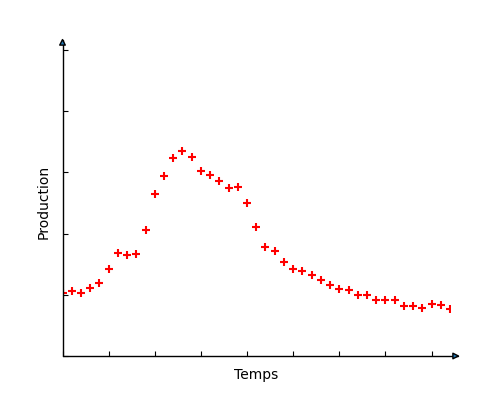
\includegraphics[width=5.5cm]{graphes/Production.png} % remplacer par le bon graphe
\end{figure}\\
$\indent$ On remarque donc qu'avec des données non bruitées, l'algorithme ne bloque pas, mais ne converge plus à partir de $a = 1$.\\

% Extremum de bruit avec éloingement nul
$\indent$ Cherchons donc le niveau de bruit limite : la valeur de $\sigma$ au delà de laquelle notre algorithme ne converge plus, même avec des paramètres initiaux très proches de la solution ($\bs{\Theta}_{init} = 1,10*\bs{\Theta}_{opti}.$)\\
% à illustrer
\begin{figure}[h]
	\center
	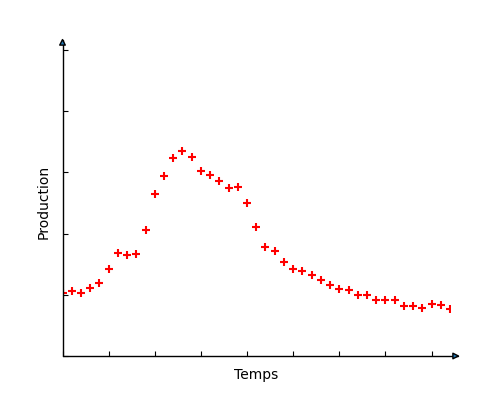
\includegraphics[width=5.5cm]{graphes/Production.png} % remplacer par le bon graphe
\end{figure} \\

$\indent$ On constate qu'avec des paramètres initiaux très proches de la solution, l'algorithme bloque à partir d'un bruit de 200. ( la matrice B est singulière )



\subsection{Performance \textit{-optionnel}}
% Test des performances de l'algorithme %
$\indent$ Testons maintenant les performances de notre algorithme de manière plus rigoureuse. 


\subsubsection{Temps de convergence selon diffèrent paramètres}
% Différents tests sur la vitesse de convergence sur par exemple :  le niveau de bruit, la distance de départ par rapport à la solution, facteur de rebroussement, etc %
Pour chaque valeurs de $\sigma$ et de $a$, nous allons lancer l'algorithme d'optimisation 100 fois et calculer les moyennes du temps d'exécution et de la valeur du critère final (l'adéquation au données du modèle obtenu).
 
% performances sur données plus ou moins bruitées avec 
\begin{figure}[h]
	\center
	\subfigure{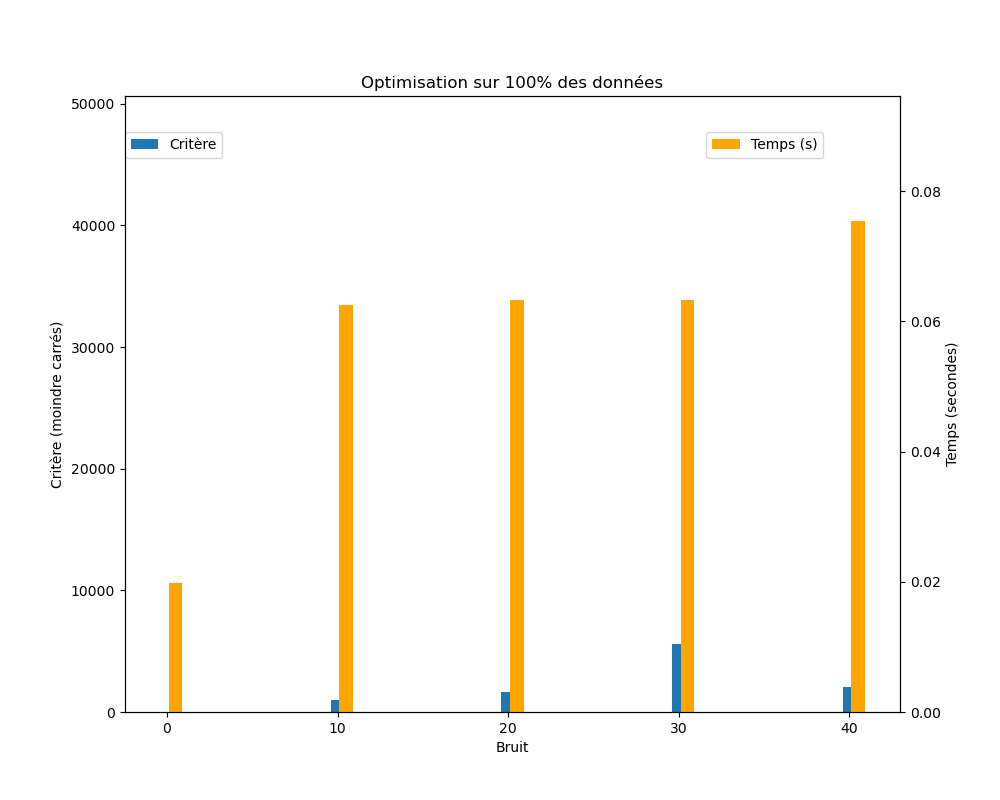
\includegraphics[width=0.45\textwidth]{graphes/performances/perfs_ModelOnGeneratedData_DataQ_100.png}}
	\subfigure{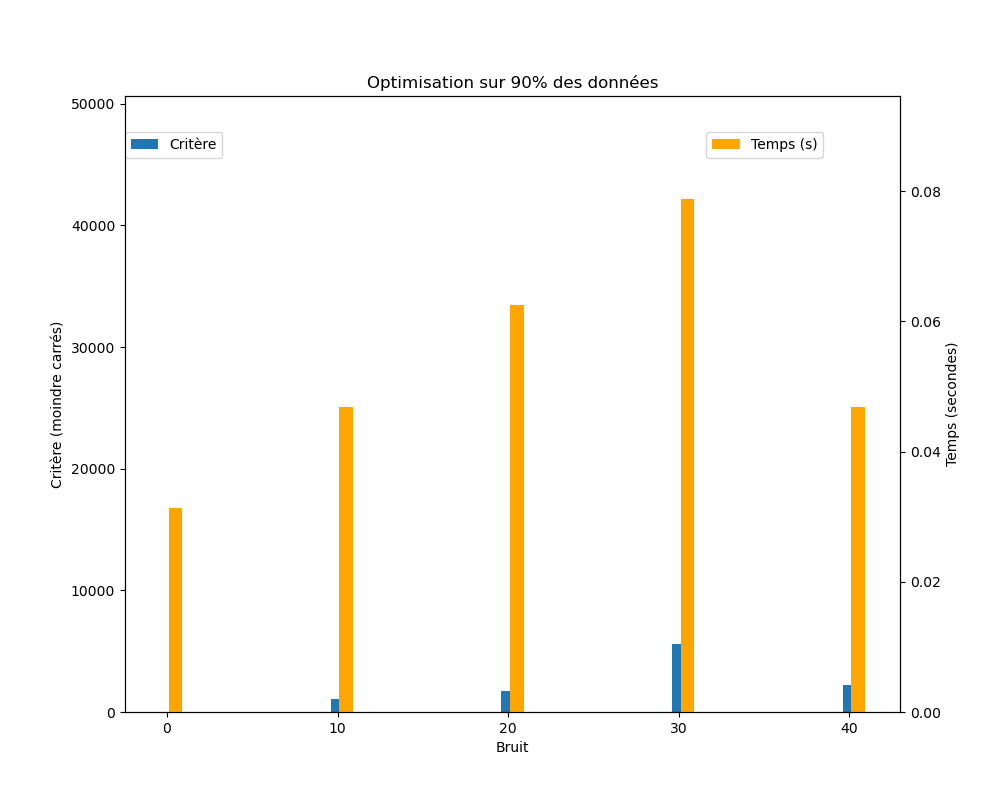
\includegraphics[width=0.45\textwidth]{graphes/performances/perfs_ModelOnGeneratedData_DataQ_90.png}}
	\subfigure{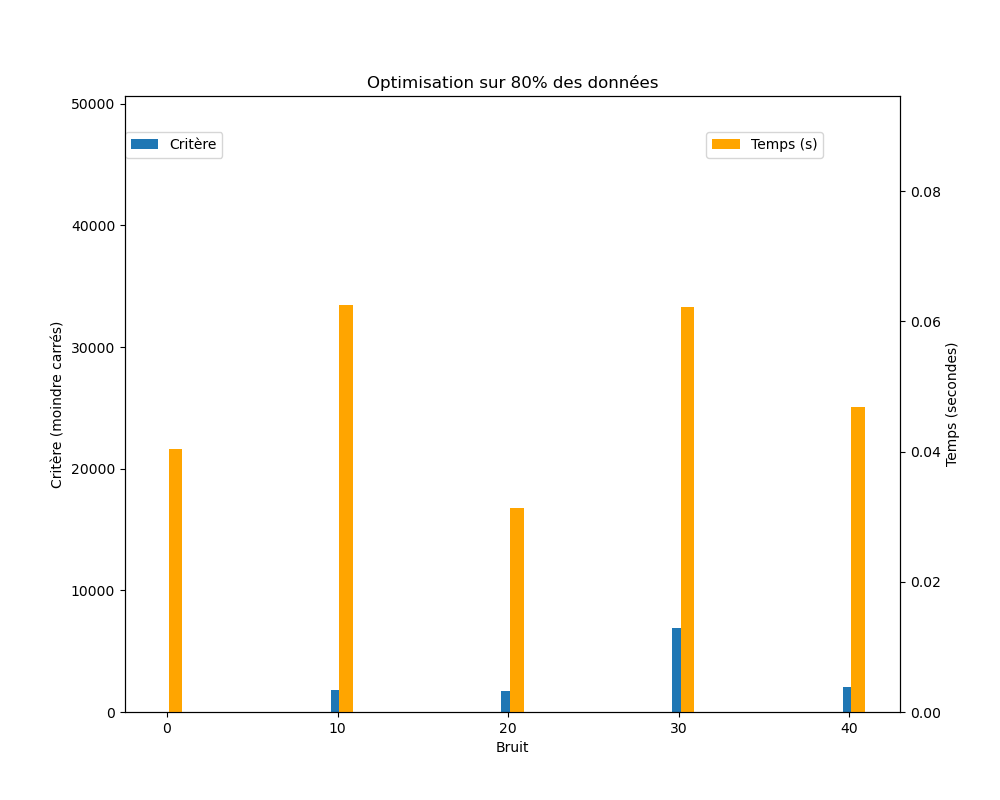
\includegraphics[width=0.45\textwidth]{graphes/performances/perfs_ModelOnGeneratedData_DataQ_80.png}}
	\subfigure{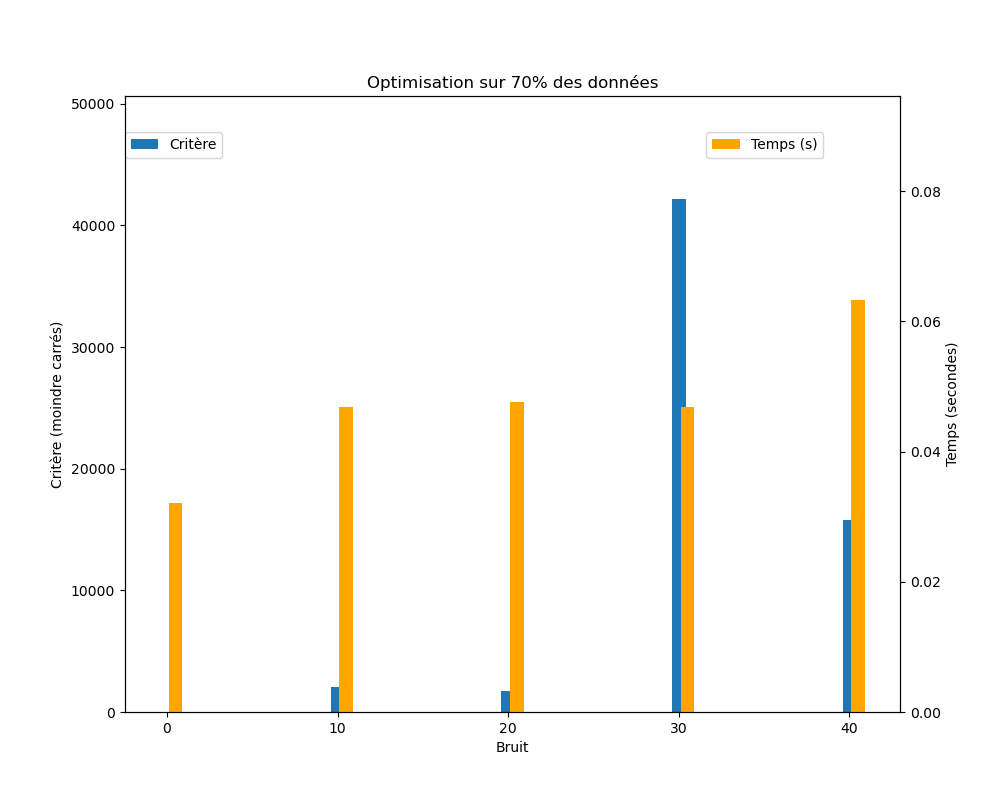
\includegraphics[width=0.45\textwidth]{graphes/performances/perfs_ModelOnGeneratedData_DataQ_70.png}}
	\caption{Temps d'exécution et critère final moyens selon différents niveau de bruitage des données initiales pour des arguments initiaux égaux à 100\%, 90\%, 80\% et 70\% des arguments de génération.}
\end{figure}

\section{Données réelles}
% Après l'introduction de l'algorithme, introduction de l'algorithme aux données réelles et évaluation des ces performances %
$\indent$ Maintenant que nous savons que notre algorithme fonctionne, voyons si le modèle qu'il génère est pertinent lorsqu'il s'agit de représenter des données réelles. Pour cela, nous utiliserons les données de production pétrolière que l'OCDE met à disposition de chacun sur son site web.

\subsection{Modélisation de la production pétrolière de la France}
% Application de l'algorithme sur un jeu de données pertinentes %
$\indent$ Essayons par exemple d'appliquer notre algorithme aux données de production pétrolière de la France. On jouant manuellement sur les paramètres, on trouve une première approximation de la sigmoide optimale :

%remplacer par la sigmoide obtenue avec les sliders
\begin{equation}\label{linspring} 
\begin{gathered}
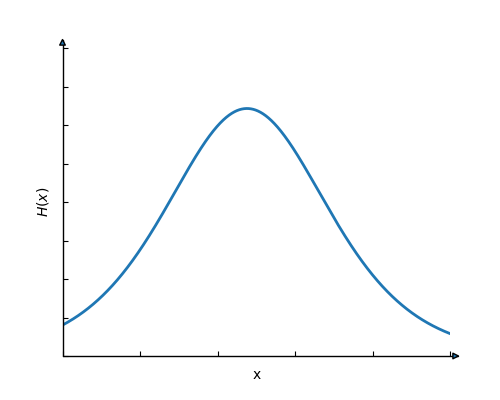
\includegraphics[width=0.40\textwidth]{graphes/CourbeHubbert.png} 
\end{gathered}
S_{75000,16,6.5}(t) 
\qquad
\end{equation}

$\indent$ Nous allons donc lancer l'algorithme avec ces paramètres initiaux. Voici le modèle que l'on obtient :

% remplacer par le graphe ploté par l'optimisation et par les paramètres rendus
\begin{equation}\label{linspring} 
\begin{gathered}
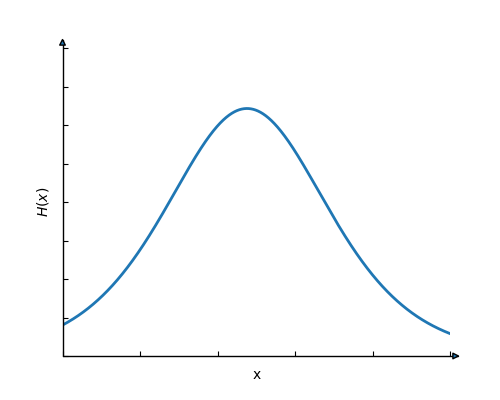
\includegraphics[width=0.40\textwidth]{graphes/CourbeHubbert.png} 
\end{gathered}
S_{75000,16,6.5}(t) 
\qquad
\end{equation}

$\indent$ Le résultat semble pertinent : il colle bien aux données et reconnait avec précision le pic de production ainsi que la quantité totale de pétrole produite. A priori, l'algorithme est assez efficace et ses résultats sont pertinents. Mais d'une part nous avons dû l'initialiser manuellement, et d'autre part, la production pétrolière de certains pays ne suit pas aussi clairement une courbe en cloche que celle de la France.

\subsection{Application de l'algorithme aux données des pays de l'OCDE}
% Généralisation du test de pertinence %
$\indent$ Essayons maintenant d'automatiser notre démarche pour la généraliser à l'ensemble des pays dont les données de production pétrolière sont présentes sur le site de l'OCDE. \\
$\indent$ Dans le cas de la France, nous avions approximé manuellement les des paramètres initiaux. Ici, afin d'automatiser le processus, nous allons définir $\bs{\Theta}_{\text{init}}$ comme suit : \\

\begin{equation}\label{linspring}
\bs{\Theta}_{\text{init}} = \left[\begin{array}{c}
S_{\text{max}} = max \left\{ D_n \right\} \\
\\
t_* = \frac{N}{2} \\
\\
\tau = 6,5
\end{array}\right]
\end{equation}
\\
$\indent$ Voici quelques cas intéressants :
\newpage
\subsubsection{Un modèle généralement pertinent}
$\indent$ La plupart des cas sont semblables à celui de la Norvège : la courbe obtenue colle relativement bien aux données, la production totale et l'année du pic sont estimés avec une marge d'erreur assez faible.\\

\begin{figure}[h]
	\center
	\subfigure{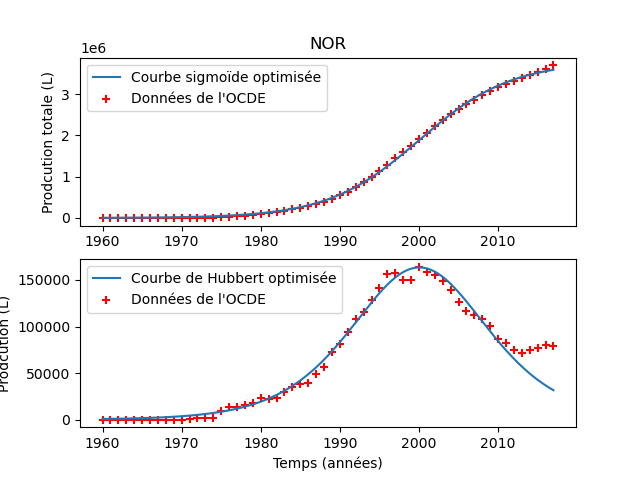
\includegraphics[width=0.45\textwidth]{graphes/Pays/NOR2022-04-26.png}}
	\subfigure{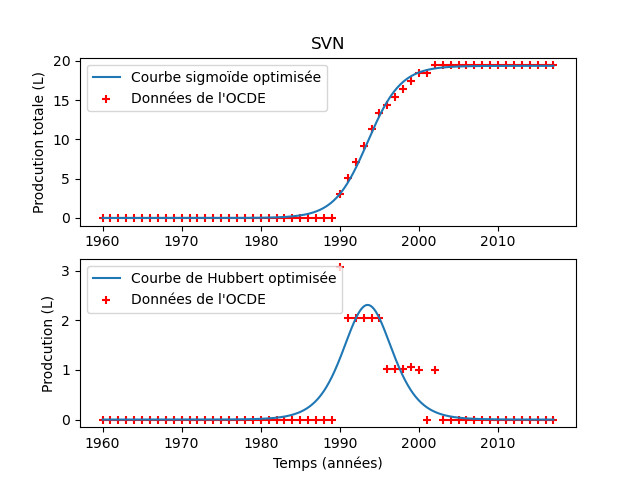
\includegraphics[width=0.45\textwidth]{graphes/Pays/SVN2022-04-26.png}}
\end{figure}


\subsubsection{Un modèle parfois inadapté}
$\indent$ Dans des pays comme l'Azerbaijan, où la production est relativement constante, le modèle s'avère sans surprise complètement inadapté.\\
  
\begin{figure}[h]
	\center
	\subfigure{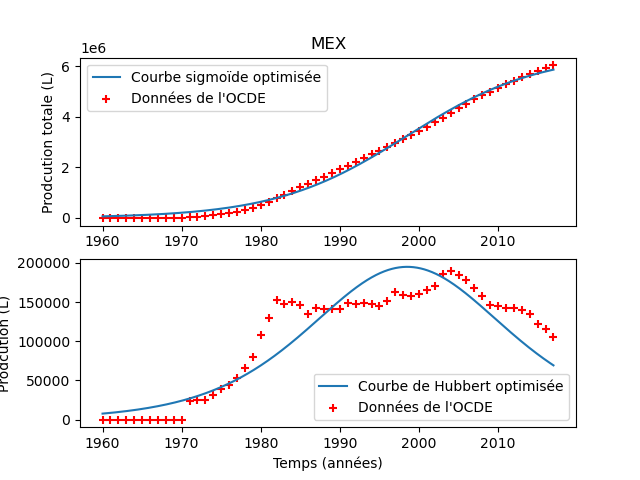
\includegraphics[width=0.45\textwidth]{graphes/Pays/MEX2022-04-26.png}}
	\subfigure{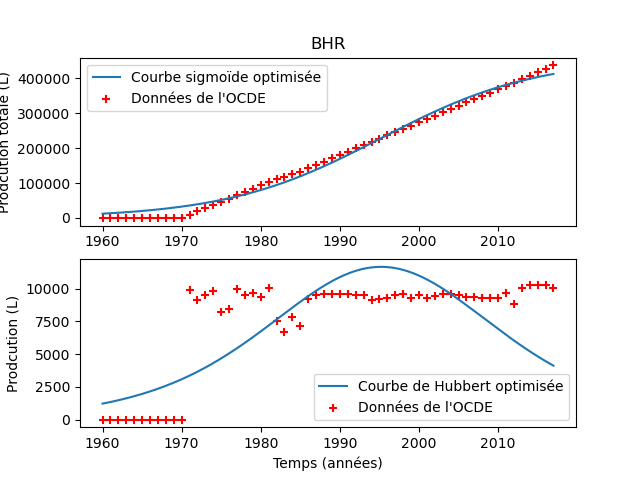
\includegraphics[width=0.45\textwidth]{graphes/Pays/BHR2022-04-26.png}}
\end{figure}
% Chercher à expliquer ce schéma de production dans ces pays


\newpage
\subsubsection{Des cas ambigus}
$\indent$ Pour certains pays, comme l'Albanie ou l'Australie, le modèle colle vaguement aux données, mais il apparait assez clairement qu'il est limité par ses hypothèses : il y a eu dans ces pays plus d'un pic de production. Néanmoins, si l'on regarde chaque pic indépendant, il ne semble pas déraisonnable de penser qu'il pourrait être modélisé par une courbe de Hubbert. Pourrait-on modifier notre modèle pour lui permettre de représenter des cas de ce genre ? Nous étudierons la question par la suite.

\begin{figure}[h!]
	\center
	\subfigure{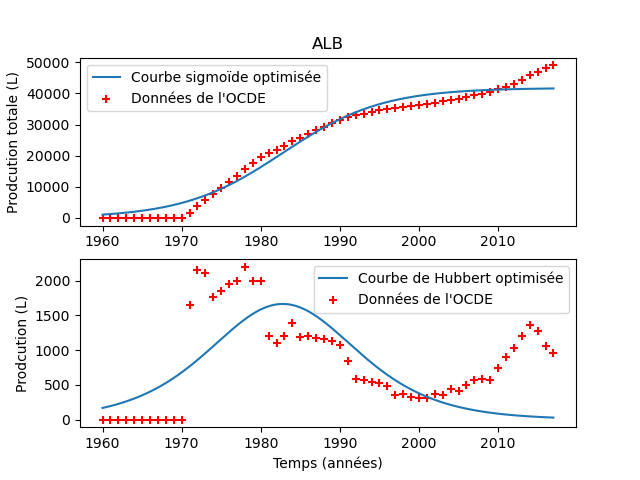
\includegraphics[width=0.45\textwidth]{graphes/Pays/ALB2022-04-26.png}}
	\subfigure{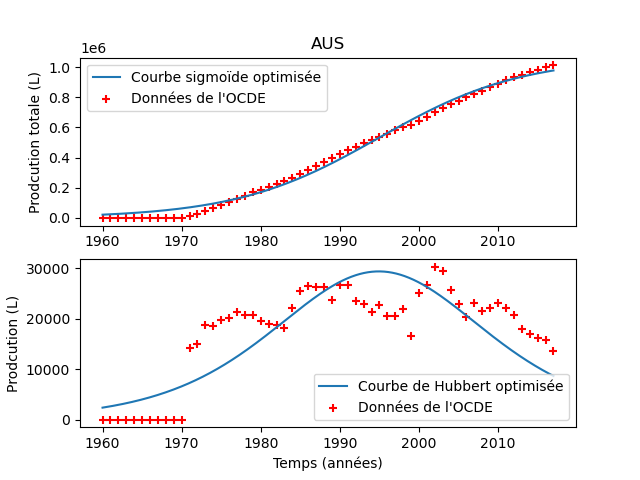
\includegraphics[width=0.45\textwidth]{graphes/Pays/AUS2022-04-26.png}}
\end{figure}


\subsubsection{ Modélisation de la production mondiale}
% Test de la pertinence du modèle sur une vue globale %
$\indent$ Qu'en est-il de la production cumulée de tous les pays de l'OCDE ? La courbe de Hubbert permet-elle d'estimer la quantité de pétrole que l'humanité entière pourrait exploiter ? Il apparait que non : la production mondiale ne semble pas vérifier l'hypothèse du pic unique et symétrique. 

\begin{figure}[h]
	\center
	\subfigure{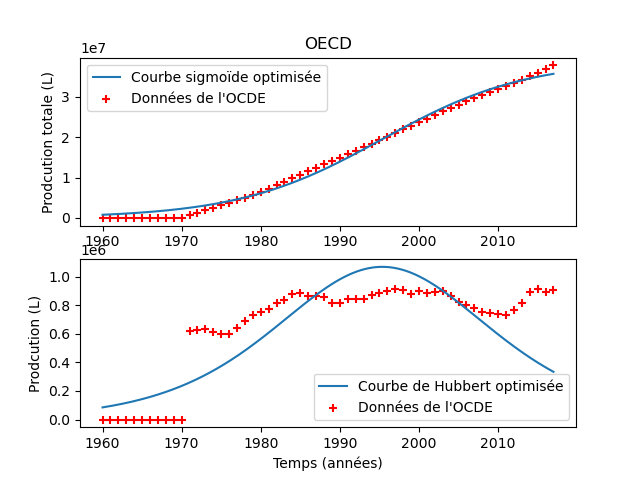
\includegraphics[width=0.7\textwidth]{graphes/Pays/OECD2022-04-26.png}}
\end{figure}





\subsection{Prévisions à partir du modèle}
% Vérification de la performance de l'algorithme pour trouver les pics de production %
$\indent$ Nous avons constaté que, lorsque certaines hypothèses sont vérifiées, le modèle de Hubbert colle relativement bien au données réelles. Cependant, modéliser des données à posteriori n'a que peu d'intérêt. Notre algorithme est-il capable de plus ? Le modèle obtenu permet-il de prédire l'évolution de la production dans une fenêtre qui dépasse celle des données sur lesquelles il a été optimisé ?


\subsubsection{Optimisation sur données incomplètes}
% La détermination du pics étant simple a posteriori, on peut calculer de la performance de l'algorithme à trouver le pic de production a posteriori %
$\indent$ Pour évaluer la capacité de notre algorithme à prévoir l'évolution de la production, nous allons le lancer sur des versions écourtées des données de l'OCDE, et comparer les prévisions du modèle obtenu aux données réelles. Nous nous limiterons bien entendu aux pays pour lesquels nous obtenions des résultats cohérents lorsque nous lancions l'algorithme sur les données complètes.\\

$\indent$ Voici ce que nous obtenons dans le cas du Danemark, par exemple :
\begin{figure}[h]
	\center
	\subfigure{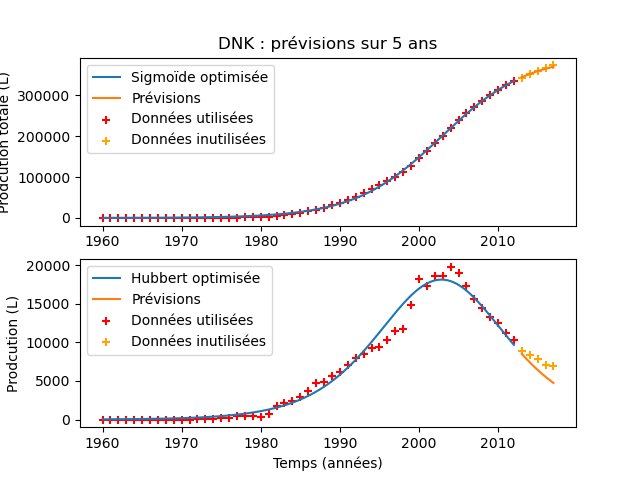
\includegraphics[width=0.45\textwidth]{graphes/Pays/previsions/prev5_DNK2022-04-27.png}}
	\subfigure{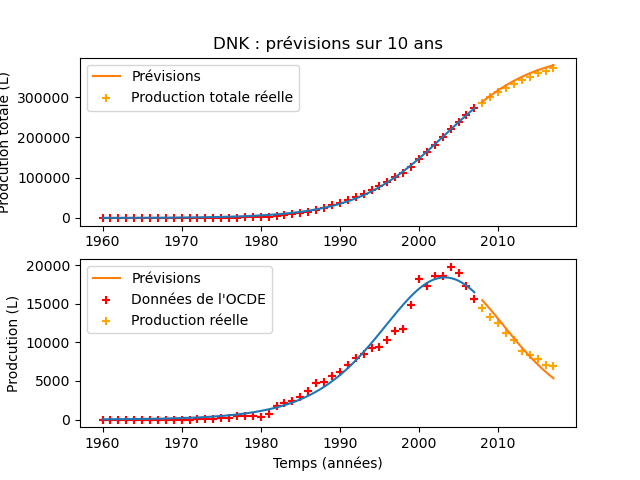
\includegraphics[width=0.45\textwidth]{graphes/Pays/previsions/prev10_DNK2022-04-27.png}}
	\subfigure{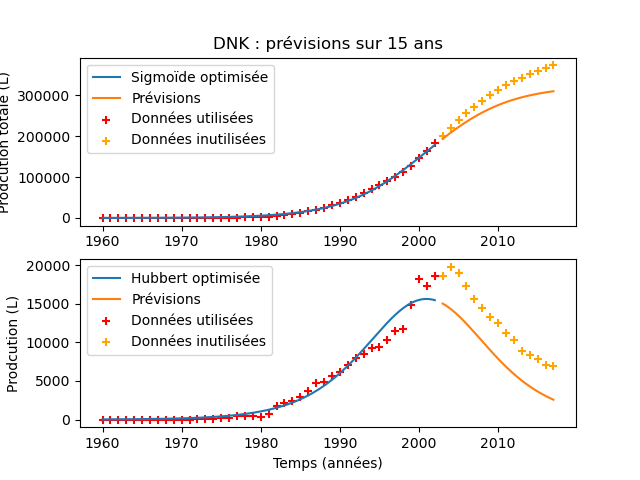
\includegraphics[width=0.45\textwidth]{graphes/Pays/previsions/prev15_DNK2022-04-27.png}}
	\subfigure{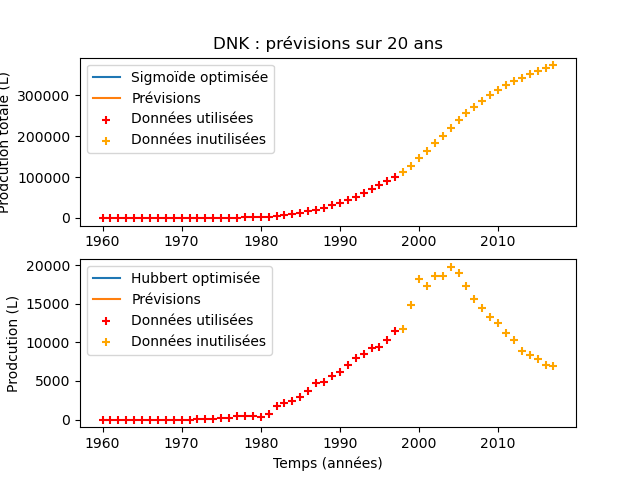
\includegraphics[width=0.45\textwidth]{graphes/Pays/previsions/prev20_DNK2022-04-27.png}}
	\caption{Prévisions de la production pétrolière du danemark sur 5, 10, 15 et 20 ans.}
\end{figure}

$\indent$ On remarque que l'algorithme ne converge pas en deçà d'une certaine quantité de données (ici, l'algorithme n'a pas été capable de prédire l'évolution de la production lorsque le pic n'avait pas encore été atteint).

\subsubsection{Capacités prédictive du modèle de Hubbert obtenu par descente de gradient}
% En prenant des sets de données qui peuvent être convenablement modélisé par une sigmoïde, on peut cherche à quel point le modèle est prédictif. Pour cela on calcul la précision avec laquelle l'algorithme prédit le pic de production en se limitant aux premières données jusqu'à un temps $t$ %
\textit{En prenant des sets de données qui peuvent être convenablement modélisé par une sigmoïde, on peut cherche à quel point le modèle est prédictif. Pour cela on calcul la précision avec laquelle l'algorithme prédit le pic de production en se limitant aux premières données jusqu'à un temps $t$}






\subsection{Les lacunes du modèle}
% Après avoir mit en exergue les lacunes sur quelques jeux de données, tentatives de caractérisations des hypothèses de validité du modèle %
$\indent$ Comme nous l'avons vu, la pertinence du modèle de Hubbert est inconstant. Si dans la plupart des cas il colle assez bien à la réalité, les cas qui le tiennent en échec ne manquent pas. Nous avons clairement défini ses hypothèses dans l'introduction :
\begin{itemize}
	\item La production de ressources premières croit, atteint un unique pic, puis décroit.
	\item Son évolution est symétrique par rapport à cet unique pic
\end{itemize}

$\indent$ L'expérience nous montre que ces hypothèse sont souvent fausses : certains pays, comme l'Albanie ou l'Australie, découvrent un nouveau gisement après avoir commencé, et potentiellement terminé, d'en exploiter un premier. D'autres, comme le Mexique, n'entrent pas dans le schéma industriel classique : la croissance initiale laisse place à la stagnation plutôt qu'à la décroissance. 


\subsection{Amélioration de modèle}
% Avec un algorithme flexible, on peut essayer d'améliorer la modélisation %
$\indent$ Le modèle de Hubbert nous donne des résultats plutôt satisfaisants, mais ses hypothèses sont assez contraignantes. Nous avons donc réfléchi à une façon de l'étendre, de sorte à ce qu'il soit applicable à des cas plus variés.

\subsubsection{ Deux sigmoïdes}
% Si il y a deux pics, est-ce que deux sigmoïdes additionnées est un bonne modélisation? %
\textit{Si il y a deux pics, est-ce que deux sigmoïdes additionnées est un bonne modélisation?}

\subsubsection{n sigmoïdes}
% Si il y a n pics, est-ce que n sigmoïdes additionnées est un bonne modélisation? %
\textit{Si il y a n pics, est-ce que n sigmoïdes additionnées est un bonne modélisation?}

\section{Conclusion}
\end{document}
